\documentclass{mscLiterature}
%
%
% Thesis data
%\mscDepartment{Delft Center for Systems and Control (\textsmaller{DCSC})}%
\mscProgram{Systems and Control}
%Change if needed to
%\mscProgram{Mechanical Engineering}
\mscFaculty{Mechanical, Maritime and Materials Engineering (3mE)}%
\mscName{Yudha Prawira Pane}%
\mscDate{\today}%
\mscTitle{Reinforcement Learning for Tracking Control in Robotics}%
%\mscSubTitle{Optional Subtitle}%
\mscKeyWords{reinforcement learning, tracking, optimal control, constraint}% only used in PDF properties
\mscCoverPicture{STYLESTUFF/COVER}% to place a picture ( here the example COVER.eps) on the back of the cover page
%
%
% Third party options (create text/logo on the copywrite page)
\mscThirdPartyText{The implementation part of the thesis is conducted at DCSC's robotics lab. The cover is courtersy of Universal Robots}
%\mscThirdPartyLogo{STYLESTUFF/EXAMPLELOGO}
% NOTE: on the title page only the TU Delft logo is permitted.
%
%
%
% Finalize the thesis data
\setThesisInfo
%
% Use \includeonly{} to build only certain parts of your thesis
%\includeonly{introduction, real_chapter, empty_chapter, long_chapter}%
%
%PH Toegevoegd 24-10-2011
%allow (matlab) listing max 1pt flexibility between lines
\lstset{lineskip=0pt plus 1pt minus 0pt}
%
\usepackage[]{algorithm2e}
\usepackage{graphicx}
\usepackage{caption}
\usepackage{subcaption}
\makeatletter
\renewcommand{\@algocf@capt@plain}{above}
\makeatother
\usepackage{tikz}
\usetikzlibrary{shapes,arrows}
\usetikzlibrary{decorations.markings}

\begin{document}
%
%========================== Front matter ======================================
\frontmatter %
%
% Make the cover page and hell of a lot of title pages
\maketitle
%
%
% Abstract (does not appear in the Table of Contents)
\chapter*{Abstract}%

Reference or trajectory tracking is one of the requirements in order to carry out a complex robotic task. Capability to perform a precise tracking with minimum possible error is crucial for the robots that are to be deployed at manufacturing industries such as semiconductor, automotive and recently, an emerging application of \ac{3D} printing.

The approach used in the past has been to design model based controllers which involve feedback and feedforward control or more recently, a predictive control. The drawback of such scheme, however, lies on the requirements of system model as a slight model mismatch could lead to poor tracking performance. For a repetitive control error, researchers have designed the so called \ac{ILC}. In this literature study, a new method to optimize the tracking performance of nominal controller using \ac{RL} is proposed. 

Throughout the literature study, the existing work for \acs{RL}-based tracking control clusters into 3 approaches: \acs{RL} for optimal tracking (Kiumarsi et al. \cite{Kiumarsi6760476}), \acs{RL}-based dynamic tuning (Brujeni et al. \cite{Brujeni5669655}), and nonlinear compensator via \acs{RL} (Bayiz et al. \cite{Efe2014}). The advantages, limitations and practical challenges of the 3 approaches are discussed. These criterion serves as a basis to select one method which will be developed and implemented during the thesis. Furthermore, the testbed for the thesis which is a UR5 \acs{3D} printing robot is also presented. Finally, the literature study concludes with the research plan and discussion.
%
% table of contents, (\toc of \toclof of \tocloflot )
\tocloflot
%
%
%
% Preface
\chapter{Preface}
This thesis came into existence after a long wander to search for a topic which suits my vision. I have always wanted to start my own robotics company some day. So the first thing that I decided was that my master thesis should have a strong practical work. To meet this goal, I set up an appointment with Subbu in his office where he explained to me about the topics which were available at the \ac {DCSC} robotics lab. At first, my topic was going to be "\ac {RL} for underactuated robot". Sounds novel and interesting. However, in terms of feasibility, this topic might become hard since there is only one underactuated robot in the lab, the slacklining robot, and it was not in a ready-to-program state. This means that I would have to spend much time making sure the robot work before I can apply my controller. Prof. Babu\v{s}ka then offers me a slightly similar topic but with totally different test bed. This is when I came into \ac {RL} for tracking control. This is a quite new topic in control field since only few people have conducted researches on it. After an hour of discussion, it is decided that this will be my thesis topic. The topic offers both theoretical and practical aspects since I will get a chance to apply my solution to a real robotic setup, UR5 from Universal Robots. Now that I am finishing my literature survey, I hope that I would deliver a satisfying result at the end of the thesis.

\vspace{30mm}
Delft, University of Technology \hfill \mscname \\
\mscdate
%
% Acknowledgements
\chapter{Acknowledgements}%

I would like to thank my supervisor Prof. Dr. Ir. R. Babu\v{s}ka for his guidance in defining my thesis topic and his valuable advices during the literature study.

I would also like to thank Subramanya Nageshrao (Subbu) for being a patient and resourceful daily supervisor. His advices help me a lot while encountering problems.

\vspace{30mm}
Delft, University of Technology \hfill \mscname \\
\mscdate
%
% Dedication page. 
\cleardoublepage
\thispagestyle{empty}
\vspace*{\stretch{1}}

\begin{quote}
\noindent``It can scarcely be denied that the supreme goal of all theory is to make the irreducible basic elements as simple and as few as possible without having to surrender the adequate representation of a single datum of experience'' 

--- \emph{Albert Einstein}
\end{quote}


\vspace{\stretch{3}}
\clearemptydoublepage
%
%========================== Main matter ======================================
\mainmatter
%
%
% Introduction
\chapter{Introduction} \label{chap::intro}
Reference or trajectory tracking is one of the building blocks to perform a complex task in robotics. Given a desired path/trajectory, the robot must be able to follow it as quickly as possible with minimum error. Capability to perform this precise tracking is crucial for robots that are to be deployed at manufacturing industries such as semiconductor, automotive, and recently, the emerging application of 3D printing. 

Statistics by International Federation of Robotics (IFR) [1] shows that the global sales of industrial robots continues to increase steadily. In 2014, it is expected that the total number of industrial robots installed reaches 205,000 units, a rise of approximately 15 \% from previous year. The survey points out that the mature markets such as automotive, electronics, and metal are responsible for such growth. 

Meanwhile, there is also a growing interests in applying robots to relatively new applications such as 3D printing, architecture, and art. For instance, research done by Gramazio et. al [2] aims to push the capability of industrial robots to make direct fabrication based on CAD model a reality. The advantage of using robots over conventional CNC machines lies on their flexibility, easy-to-adapt feature, and high degree of freedom (DOF) to enable execution of difficult configuration in 3D space. These aforementioned applications demands high precision since a minuscule of error could lead to a defect product or even worse, a disaster. Therefore, a precise, accurate reference tracking capability is inevitable.

In order to achieve this, a tracking controller is needed. However, robots are identical with non-linearities, noises, and external disturbances that are difficult to model, let alone compensate. This unknown properties often hinders the controller to perform optimally. A class of controllers which solely depends on the system's model will surely suffer a poor tracking accuracy. The natural answer to this problem is to introduce a controller capable of adjusting its parameter overtime by comparing the reference to the actual trajectory. By doing so, the controller will have an extra degree of freedom to compensate for the unknown properties hence improves the tracking quality. The controller of such characteristic belongs to the class of adaptive controller.

In this thesis, a method to improve the performance of nominal controller by using reinforcement learning (RL) is proposed. Although its existence has been since ..., the use of RL for reference tracking task in robotics is still a relatively unexplored topic. Based on the literature, there are three most notable methods of exploiting RL for tracking problem. Lewis and his group has been developing an extensive research on RL for solving the solution to adaptive optimal control. Their research has been extended for discrete and continuous time and for linear and non-linear system [4]-[6]. Bayiz et. al. has recently proposed a different approach by using RL to learn disturbance compensation for nonlinear system [4]. This disturbance compensation acts as an additive input signal to the system. The limitation of this, Finally, the    using Having the motivation of this thesis, now we are ready to define the problem to be solved/answered.



\section{Problem Definition}
The fundamental problem in this literature study concerns with the non-optimal performance of nominal controller with respect to reference tracking task. Therefore the research question can be raised as follows.

\textit{"Is it possible to integrate Reinforcement Learning technique to a nominal controller in a certain structure such that reference tracking performance of the controlled system significantly improves?"}

While conducting a research, it is considered wise to restrict oneself to a simpler context, but still captures the essential elements of the original problem. Therefore, in answering this question, some general assumptions are made.

\begin{enumerate}
	\item The system to be controlled is fully actuated
	\item The system to be controlled is both controllable and observable
	\item Nominal, stabilizing controller is available	
	\item Identification reveals some information about the system, but not adequate in order to design an accurate reference tracking controller.
\end{enumerate}

\section{Goal of the Thesis}

The goal of this thesis are as follows:
\begin{enumerate}
\item To provide a general framework of improving tracking control using RL
\item To apply and compare existing method of RL for tracking application to the 3D printing robotic setup
\item To come up with modification of improvement of previous methods
\end{enumerate}

\section{Literature Study Approach}
In order to build a strong theoretical foundation for later implementation, the following literature approach is used. The order does not necessarily represent a sequential process.
\begin{enumerate}
	\item To gather as many relevant papers as possible from reputable academic search engines. Relevant means papers which deal with RL and control system. Additional pointer to tracking problem is heavily considered. Examples of sources being used are Web of Science, IEEE Xplore and Google Scholar.
	\item To discuss the detail of future experimental setup (UR5 3D printing robot) with Marco de Gier, who was working on the setup at the time this literature is written.
	\item From the papers, extract existing methods which have the potential for application to the future experiments. So far, there are 3 different methods that are considered. These methods will be explained in detail in chapter 3.
	\item Program simple simulation showing the of each method
	
\end{enumerate}


\section{Outline}

The structure of this literature review is arranged as follows. In the next chapter, an introductory materials of RL is presented. This covers the framework widely used in RL (Markov Decision Process), the principle of value and policy iteration, the formulation of RL for continuous space, and the actor-critic structure which suits the framework of control system. Chapter 3 provides the result of literature study being conducted. This includes the detailed explanation of methods found and their comparison. Furthermore, a new controller is proposed. 

\section{Nomenclature}



\chapter{Reinforcement Learning Preliminaries}
This chapter is dedicated to present a concise theory of reinforcement learning. The first section will show how a certain goal can be formalized as a reward maximization -- one of the ideas which serves as a basic foundation of \ac{RL}. Section \ref{sec:mdp} explains the basics of \ac{MDP}, a general framework used in \ac{RL} problem. The notion of value function will be discussed in Section \ref{sec:value}. Subsequently, a method to solve \ac{RL}, namely policy and value iteration will be developed in section \ref{sec:value_iter}. Finally, Section \ref{sec:actor} will discuss the actor-critic structure which is an alternative solution to policy iteration.

\section{Goal as Cost Minimization}
The nature of \ac{RL} is inspired by the way living organisms learn to reach their desired goals. Animals for instance, learn by first acting on the environment, observe the changes that occur, and improve their action iteratively. One example is a circus lion that is tasked to perform acrobatic show while its trainer observing the progress. If the lion successfully executes the task, it will be rewarded with foods. Conversely, punishment will be inflicted whenever it fails. The lion initially has no idea of how to perform the task. However through trial and error, it will follow its instinct to increase the frequency of receiving rewards while trying its best to avoid punishments. In a certain duration of training, the circus lion will be finally able to perform the task flawlessly. 

Now we will formalize above illustration for robotics application. A robot can be described by its states $x_k$ with subscript $k$ denoting time instance. Applying an action $u_k$ will bring the robot to state $x_{k+1}$ with immediate reward $r_{k+1}$. Subsequently, at $k+1$ the robot applies $u_{k+1}$ which yields state $x_{k+2}$ and $r_{k+2}$. This action-state-update iteration is run for infinite time instances. The goal is defined as maximization of cumulative reward the robot receives. In control engineering, reward is usually replaced with cost. In that case the goal is defined as minimization problem. Starting from now, we will define goal as minimization of future cost $J$.

From the sequence of cost obtained over time, we can define a formalization of goal, called expected return. Return $J_t$ is a function that maps the sequence of costs into real number. An example of return is the sum of the costs:

\begin{equation}
J_t = r_{t+1} + r_{t+2} + r_{t+3} + \dots + r_T
\end{equation} 

\section{Markov Decision Process} \label{sec:mdp}
\ac{MDP} is defined as a tuple $\left<X, U, f, \rho \right>$ which satisfies Markov property \cite{babuskaRL}. The detailed explanation of Markov property can be found on \cite{sutton1998reinforcement} section 3.5 but the main idea is that to determine the probability of a state at certain time, it is sufficient to only know the state of previous time instance. The elements of the tuple are:
\begin{itemize}
	\item $X$ is the state space
	\item $U$ is the action space
	\item $f :X \times U \rightarrow X$ is the state transition function (system dynamics) 
	\item $\rho:X \times U \rightarrow \mathbb{R}$ is the reward function
\end{itemize}

In control engineering, $f$ represents the system dynamics which is a transition function mapping a current state and action to the one-step ahead state up to a probability distribution. This probability distribution is mathematically denoted as

\begin{equation}
	\text{Pr}\{x_{t+1} = x', r_{t+1} = r| x_t, u_t \}
	\label{eq:markov}
\end{equation}
where $x$ denotes state, $u$ denotes action, and $r$ denotes immediate reward obtained upon applying the input on the corresponding state. 



\section{Value Function} \label{sec:value}
Value function describes how good a particular state or state-action pair under a certain policy. As previously explained, in this thesis we will stick to control engineering convention by seeing \ac{RL} as cost minimization problem. Therefore, the smaller value function of a state $x$, the better it is. The value function is denoted by $ V^{\pi}(x) $ for state-value function and $ Q^{\pi}(x,u) $ for action-value function under policy $\pi$. It can be written in terms of immediate reward and the value function of the next state by following derivation
\begin{equation}
\begin{split}
V^{\pi}(x_t) &= \rho(x_t,u_t) + \gamma \rho(x_{t+1},u_{t+1}) + \gamma^2 \rho(x_{t+2},u_{t+2}) + ... + \gamma^{\infty}\rho(x_{\infty},u_{\infty}) \\
V^{\pi}(x_t) &= \rho(x_t,u_t) + \gamma \left( \rho(x_{t+1},u_{t+1}) + \gamma^2 \rho(x_{t+2},u_{t+2}) + ... + \gamma^{\infty}\rho(x_{\infty},u_{\infty})\right)  \\
V^{\pi}(x_t) &= \rho(x_t,u_t) + \gamma V^{\pi}(x_{t+1})
\end{split}
\end{equation} 

Furthermore, one can always find a policy which gives an optimal value function $V^*$. This optimal value function respects the Bellman optimality equation, which can be written as 
\begin{equation}
V^*(x_t) = \rho(x,u) + \gamma \min_{u} V^*(x_{t+1})
\label{eq:bellman}
\end{equation}
Similarly, the action-value function is

\begin{equation}
Q^*(x_t,u_t) = \rho(x,u) + \gamma \min_{u} Q^*(x_{t+1},u_{t+1})
\label{eq:bellman2}
\end{equation}

Discount factor $\gamma$ is introduced to avoid the value function goes to infinity. Once $V^*$ is known, the optimal policy can be taken in a greedy way as
\begin{equation}
\pi^* = \text{arg} \max_{\pi} V^*(x)
\label{eq:optPi}
\end{equation}
This concludes the formulation of \ac{RL} problem. The subsequent sections will deal with two methods to solve for the solution.

\section{Policy and value iteration} \label{sec:value_iter}
\ac {PI} and \ac{VI} belong to a class of elementary solution to the \ac{RL} called  dynamic programming \cite{sutton1998reinforcement}. They are characterized by the requirement of system model $f$. These methods are closely related with a branch of control system, namely optimal control \cite{126844}.

\ac {PI} is a two steps algorithm, consists of policy evaluation and policy improvement. Let the initial policy at certain state $x$ be given by $ \pi$. A better policy can be determined by first evaluating the old policy's value $ V^{\pi} $, search for the optimal action at state $x$ greedily, and replace the old policy with the optimal action. This process can be casted as Algorithm~\ref{alg:PI}. Note that the policy evaluation step is actually a Bellman equation \eqref{eq:bellman} turned into assignment. The \textit{policy-stable} variable is to indicate that the policy does not change anymore i.e. converged.

\begin{algorithm}
	\textbf{Initialization:} \\
	Start from an admissible policy $ \pi $\\
	Initialize $V^{\pi}(x)$ arbitrarily, e.g. $ V^{\pi}(x) = 0 \hspace{2mm}  \forall x \in \mathcal{X} $ \\
	\Repeat(){\textit{policy-stable} = true}{	
	\textbf{Policy Evaluation:} \\
		\Repeat(){$ \Delta  <  \varepsilon $ (a small positive number)}{
		$ \Delta $ $ \leftarrow $ 0 \\
		\textbf{For each} $ x \in \mathcal{X} $ :\\
			\hspace{5mm} $ v $ $ \leftarrow $ $ V^{\pi}(x) $ \\
			\hspace{5mm} $ V^{\pi}(x) \leftarrow \rho(x, \pi(x)) +\gamma V^{\pi}(x') $ \\
			\hspace{5mm} $ \Delta = $ max$ (\Delta, |v-V^{\pi}(x)|) $ \\}
			\vspace{2mm}
	\textbf{Policy Improvement:} \\
		\textit{policy-stable} $ \leftarrow $ false \\
		\textbf{For each} $ x \in \mathcal{X} $ : \\
			\hspace{5mm} $ b \leftarrow \pi(x) $ \\
			\hspace{5mm} $ \pi(x)=$  arg $\underset{u}{\text{min}} \hspace{1mm} \rho(x, u) +\gamma V^{\pi}(x') $  \\
			\hspace{5mm} \textbf{if} $ b = \pi(x) $ \textbf{then} \\ 
			\hspace{10mm} \textit{policy-stable} $ \leftarrow $ true \\
			\hspace{5mm} \textbf{endif}
	}
\caption{Policy iteration algorithm}
\label{alg:PI}
\end{algorithm}

\ac{VI} is similar to, but more efficient version than \ac{PI}. In order to increase computational efficiency, instead of evaluating value function $V$ for all possible state $x$ in every iteration, one can evaluate the value function in greedy way, which results in less iteration. Once the value function converges to $V^*$, the optimal policy can be directly obtained as the control input which minimizes $V$. This algorithm is shown in Algorithm~\ref{alg:VI}. 

\begin{algorithm}
	\textbf{Initialization:} \\
	Start from an admissible policy $ \pi $\\
	Initialize $V^{\pi}(x)$ arbitrarily, e.g. $ V^{\pi}(x) = 0 \hspace{2mm}  \forall x \in \mathcal{X} $ \\
	\Repeat(){policy converges to $ \pi^* $}{
		\Repeat(){$ \Delta  <  \varepsilon $ (a small positive number)}{
			$ \Delta $ $ \leftarrow $ 0 \\
			\textbf{For each} $ x \in \mathcal{X} $ :\\
			\hspace{5mm} $ v $ $ \leftarrow $ $ V^{\pi}(x) $ \\
			\hspace{5mm} $ V^{\pi}(x) \leftarrow \underset{u}{\text{min}} \rho(x, \pi(x)) + \gamma V^{\pi}(x') $ \\
			\hspace{5mm} $ \Delta = $ max$ (\Delta, |v-V^{\pi}(x)|) $ \\}
		\vspace{2mm}
		Obtain a deterministic policy: \\
		$ \pi(x)=$  arg $\underset{u}{\text{min}} \hspace{1mm} \rho(x, u) +\gamma V^{\pi}(x') $  \\

	}
	\caption{Value iteration algorithm}
\label{alg:VI}
\end{algorithm}

 
\section{Actor Critic Method} \label{sec:actor}
The second method for solving \ac{RL} is by using temporal-difference learning. It is favored due to its model-free nature. In this section, we will discuss a class of \ac{TD} called actor-critic method. The idea of actor-critic method is to separate policy and value function into entities called actor and critic respectively (see Figure~\ref{fig:actorCritic}). The critic evaluates and criticizes the actor performance by feeding a temporal difference signal $\delta$ to the actor. This signal is basically the difference between right and left hand side of Bellman equation, in other words, the Bellman equation error. 

In order to deal with continuous state space, the actor $\psi$ and critic $\theta$ functions are parameterized by function approximators. Examples of function approximators are fuzzy, neural networks and tile coding. The actor-critic method is presented in Algorithm~\ref{alg:actorcritic} (adapted from \cite{babuskaRL}). Note that $\tilde{u}$ denotes random exploration term which is needed to avoid getting stuck at local optimum.

\begin{figure}[h!]
\centering
\includegraphics[width=0.6\linewidth]{actorCritic2}
\caption{Actor critic structure (diagram reproduced from \cite{babuskaRL})} 
\label{fig:actorCritic}
\end{figure}

\begin{algorithm}
	\For{every trial}{
		Initialize $x_0$ and $u_0 = \tilde{u}_0$\\
		\Repeat{terminal state}{
			apply $u_k$, measure $x_{k+1}$, receive $r_{k+1}$ \\
			choose next action $ u_{k+1} = \hat{\pi}(x_{k+1}, \psi_k)	+ \tilde{u}_{k+1} $ \\
			$ \delta_k = r_{k+1} + \hat{V}(x_{k+1}, \theta_k) - \hat{V}(x_{k}, \theta_k) $ \\
			$ \theta_{k+1} = \theta_k + \alpha_c\delta_k \frac{\partial \hat{V}(x,\theta)}{\partial \theta} \bigg|_{x=x_k, \theta = \theta_k}$ \\
			$ \psi_{k+1} = \psi_k + \alpha_c\delta_k \frac{\partial \hat{V}(x,\psi)}{\partial \psi} \bigg|_{x=x_k, \psi = \psi_k}$
		}
	}
	\caption{Actor-critic algorithm}
	\label{alg:actorcritic}
\end{algorithm}



%
% A Real Chapter
\chapter{Reinforcement Learning for Tracking Problem: A Survey} \label{chap::survey}
Despite the success of \acs{RL} in many robotics problem (e.g. learning to fly \cite{Abbeel}, walk \cite{NIPS2007_3253} and navigate \cite{4543641}), the application of \acs{RL} for tracking control is not a widely explored topic. Over the spans of the literature survey, author finds several attempts to exploits \acs{RL} for tracking problem, which can be categorized into 3 different approaches: dynamic tuning, \acs{RL} for optimal control, and \acs{RL} for nonlinear additive compensator. 

This chapter covers the foundational theory of the 3 aforementioned approaches. The main idea, advantages, limitations and ease of implementation are the key issues which will be discussed in the next chapter. These issues will serve as the basis of the argument to choose one method for later implementation. The chapter starts in Section \ref{sec:rl_lqt} by providing explanation about \acs{RL} for optimal tracking control. Section \ref{sec:dytun} deals with the so called dynamic tuning -- a class of gain scheduling which makes use of \acs{RL}. The third method, presented in Section \ref{sec:nl_comp}, is a relatively new approach which employs \acs{RL} to learn additive input compensation.


\section{Reinforcement Learning for Optimal Tracking Control} \label{sec:rl_lqt}
This method is initiated and developed by Lewis et. al. which aims to solve the tracking by \acs{RL} problem from dynamic programming perspective. The method uses optimal control, a branch of control theory whose root is closely related to dynamic programming \cite{126844}. The method starts from the downside of optimal tracking control which requires the solution of non-causal differential equation. It turns out that by assuming the reference to follow a certain dynamics and modifying the state of the optimal tracking, a causal representation can be obtained. Once a causality is in hand, we can then employ our favorite \acs{RL} techniques to asymptotically solve for the solution. 

To provide an easier comparison between the standard optimal tracking solution with \acs{RL}-based one, this section starts by formulating the standard optimal tracking problem and deriving its solution. Next, the modified formulation of optimal tracking which allows the causal formulation of infinite horizon optimal tracking problem is discussed. Following is the \acs{PI} algorithm to solve the optimal tracking. In this section, only discrete-time \ac{LQT} problem is considered \cite{Kiumarsi6760476}. Although the extension to non-linear and continuous time optimal tracking problem is not straightforward, the main steps are actually quite similar. The derivation presented in this section is based on work by Kiumarsi-Khomartash \cite{Kiumarsi6760476} with modifications to comply with the convention used in this report.

\subsection{Standard \acs{LQT} problem}
The standard \acs {LQT} problem is treated extensively in \cite{lewis1995optimal}. First, we formulize the \ac {LTI} discrete-time system as 

\begin{equation} \label{eq:ss}
\begin{split}
x(k+1) &= Ax(k) + Bu(k) \\
y(k) &= Cx(k)
\end{split}
\end{equation}

where $x(j) \in \mathbb{R}^n$, $u(j) \in \mathbb{R}^m$ and $y(j) \in \mathbb{R}^l$ are the state, input and output at time instance $j$ respectively. While $A$, $B$, $C$ are the state matrices. For the sake of simplicity, we omit the feedthrough matrix $D$ and consider a \ac {SISO} system. The value of a certain state $x(k)$ and reference signal $r(k)$ can be formulized as the following infinite-horizon cost function

\begin{equation}
\label{eq:infcost}
J = V(x(k), r(k)) = \frac{1}{2} \sum_{i=k}^{\infty} (Cx(i)-r(i))^TQ(Cx(i)-r(i)) + u(i)^TRu(i)
\end{equation}

where $Q \geq 0$ and $R > 0$. The goal of \acs {LQT} is to obtain the optimal tracking input $u^*(k)$ which minimizes $J$. This control input is given as a combination of feedback and feedforward term
\begin{equation}
u(k) = -Kx(k) + K_vv(k+1)
\end{equation}
where $v(k+1)$ can be obtained by solving a non-causal difference equation
\begin{equation}
v(k) = (A-BK)^Tv(k+1) + C^TQr(k)
\label{eq:noncausal}
\end{equation}
The control gains $K$ and $K_v$ are

\begin{equation}
K = (B^TSB + R)^{-1}B^TSA
\end{equation}

\begin{equation}
K_v = (B^TSB + R)^{-1}B^T
\end{equation}

where $S=S^T>0$ is a unique solution of the \ac {ARE} as follows

\begin{equation}
\begin{split}
S &= A^TS(A-BK) + C^TQC \\
&= A^TSA - A^TSB(B^TSB+R)^{-1}B^TSA + C^TQC
\end{split}
\end{equation}
Applying the optimal tracking input $u^*(k)$ gives us the minimal cost (optimal value) given by

\begin{equation}
J^* = V^*(x(k), r(k)) = \frac{1}{2}x(k)^TSx(k) - x(k)^Tv(k) + w(k)
\end{equation}

where $ w(k) $ is obtained from a backward recursion

\begin{equation}
w(k) = w(k+1) + \frac{1}{2}r(k)^TQr(k) - \frac{1}{2}v(k+1)^TB(B^TSB+R)^{-1}B^Tv(k+1)
\end{equation}

Clearly, the drawback of standard optimal tracking control is the necessity to solve a non-causal difference equation \eqref{eq:noncausal}. However, by assuming the reference trajectory to follow a certain dynamics, we can obtain a causal equation. This will be the subject of next subsection.

\subsection{Causal Representation of the \acs{LQT}}
First, the necessary assumption is that the reference is generated by following stable difference equation
\begin{equation}
r(k+1) = Fr(k) 
\end{equation}
where $ F $ is hurwitz. By augmenting the state in \eqref{eq:ss}, we obtain the following new state space system

\begin{equation}
\begin{split}
\left[ \begin{array}{c}
x(k+1) \\ 
r(k+1)
\end{array} \right] &= \left[\begin{array}{cc}
A & \textbf{0} \\ 
\textbf{0} & F
\end{array}  \right] \left[ \begin{array}{c}
x(k) \\ 
r(k)
\end{array} \right] + \left[ \begin{array}{c}
B \\ 
\textbf{0}
\end{array} \right] u(k) \\
X(k+1) &= TX(k) + B_1u(k)
\end{split}
\end{equation}

Next, we assume that the candidate lyapunov function $V$ for the augmented state space system to be

\begin{equation}
\label{eq:lqtlyap}
V(x(k), r(k)) = V(X(k)) = \frac{1}{2}X(k)^TPX(k)
\end{equation}

where $ P = P^T > 0 $

Modifying the infinite-horizon cost function \eqref{eq:infcost}, we come up with a Bellman equation for \acs{LQT}.
\begin{equation}
\begin{split}
V(x(k), r(k)) = &\frac{1}{2} (Cx(k)-r(k))^TQ(Cx(k)-r(k)) + u(k)^TRu(k) + \\
&\frac{1}{2} \sum_{i=k+1}^{\infty} \left[ (Cx(i)-r(i))^TQ(Cx(i)-r(i)) + u(i)^TRu(i)\right] 
\end{split}
\end{equation}

\begin{equation}
\begin{split}
V(x(k), r(k)) = &\frac{1}{2} (Cx(k)-r(k))^TQ(Cx(k)-r(k)) + u(k)^TRu(k) + \\
& V(x(k+1), r(k+1))
\end{split}
\end{equation}

Inserting the lyapunov equation \eqref{eq:lqtlyap}, the \acs {LQT} Bellman equation becomes
\begin{equation}
\label{eq:lqtbellman}
X(k)^TPX(k) =  X(k)^TQ_1X(k) + u(k)^TRu(k) + X(k+1)^TPX(k+1)
\end{equation}
where

\begin{equation}
Q_1 = \left[ \begin{array}{cc}
C^TQC & -C^TQ \\ 
-QC & Q
\end{array} \right] 
\end{equation}

From the \acs {LQT} Bellman equation, one can compute the time derivative (skipped here) to obtain the \acs {LQT} ARE.
\begin{equation}
\label{eq:lqtare}
Q_1 - P + T^TPT - T^TPB_1(R+B_1^TPB_1)^{-1}B_1^TPT = 0
\end{equation}

Solving for $P$ that satisfies \eqref{eq:lqtare}, we finally obtain the optimal policy 
\begin{equation}
\label{eq:opt_u}
u(k) = -K_1X(k)
\end{equation}
with
\begin{equation}
K_1 = (R+B_1^TPB_1)^{-1}B_1^TPT
\end{equation}
Our next objective is to compute $P$ of \eqref{eq:lqtare} in iterative manner using \acs {RL} instead of direct computation which might be unfeasible. 

\subsection{\acs{RL} for Solving the \acs {LQT} \acs{ARE}}
In this subsection, we will employ iterative learning algorithms to solve for $P$. Before that, we need to derive for the lyapunov equation from the \acs {LQT} Bellman equation \eqref{eq:lqtbellman} by inserting the optimal \eqref{eq:opt_u}. This yields
\begin{equation*}
X(k)^TPX(k) =  X(k)^TQ_1X(k) + X(k)^TK_1^TRK_1X(k) + X(k)^T(T - B_1K_1)^TP(T - B_1K_1)X(k)
\end{equation*}
\begin{equation}
\label{eq:lyap_lqt}
\Leftrightarrow  P =  Q_1 + K_1^TRK_1 + (T - B_1K_1)^TP(T - B_1K_1)
\end{equation}

It turns out that by choosing a stabilizing initial policy $u^0 = -K_1^0X(k)$, one can use policy evaluation and iteration to approximate $ P $. In each iteration, the policy is guaranteed to be stable. The prove of this key theorem is given in \cite{1099755}. 

By taking this theorem, one can design both offline and online \acs{PI} algorithms to asymptotically approximate $P$. The offline \acs{PI} improves $P$ using the lyapunov function \eqref{eq:lyap_lqt}, while the \acs {LQT} Bellman equation \eqref{eq:lqtbellman} is used for the online \acs{PI}. These two algorithms are listed in Algorithm~\ref{alg:off_pi} and \ref{alg:on_pi}. We can see that for the offline \acs{PI}, we can directly obtain $P$. Meanwhile, for the online \acs{PI}, $P$ needs to be solved with a least square method. Note that both require the knowledge of the system dynamics. If the model is not (fully) known, one can use Q-learning \cite{Kiumarsi20141167} or actor-critic \acs {RL} \cite{Modares20141780} instead. 

\begin{algorithm}[H]
	%	\KwData{this text}
	%	\KwResult{how to write algorithm with \LaTeX2e }
	\textbf{Initialization:} Select an admissible (stable) gain $K^0_1$\\
	\Repeat(){$ P $ converges}{
		\textbf{Policy evaluation:} \\
		$P^{j+1} = Q_1 + (K_1^j)^TRK_1^j + (T-B_1K_1^j)^TP^{j+1}(T-B_1K_1^j)$\\
		
		\textbf{Policy improvement:} \\
		$ K_1^{j+1} = (R+B_1^TP^{j+1}B_1)^{-1} B_1^TP^{j+1}T $\\	
	}
	\label{alg:off_pi}
	\caption{Offline Policy Iteration}
\end{algorithm}

\begin{algorithm}[H]
	%	\KwData{this text}
	%	\KwResult{how to write algorithm with \LaTeX2e }
	\textbf{Initialization:} Select an admissible (stable) gain $K^0_1$\\
	\Repeat{$ P $ converges}{
		\textbf{Policy evaluation:} \\
		$X(k)^TP^{j+1}X(k) = X(k)^T\left( Q_1 + (K_1^j)^TRK_1^j\right) X(k) + X(k+1)^TP^{j+1}X(k+1)$\\
		
		\textbf{Policy improvement:} \\
		$ K_1^{j+1} = (R+B_1^TP^{j+1}B_1)^{-1} B_1^TP^{j+1}T $\\	
	}
	\label{alg:on_pi}
	\caption{Online Policy Iteration}
\end{algorithm}

\subsection{\acs{RL} for \acs{LQT} with unknown system dynamics}
As the main goal of this thesis is to improve reference tracking by compensating for the unknown dynamics using \acs {RL}, the previously descibed \acs {PI} method which requires full information about the system dynamics is no longer relevant. In order to relax this requirement, we will turn to \acs {TD} learning. The solution to optimal tracking problem for a partially unknown system is given in \cite{Kiumarsi6760476} \cite{Kiumarsi6918527} and \cite{Modares20141780}. Although the method no longer requires drift dynamics $T$, input dynamics $B_1$ is still necessary. For a fully unknown system dynamics, a method proposed in \cite{Kiumarsi20141167} is the solution. 

We start by first defining the Q function as 
\begin{equation}
Q(X(k), u(k)) = \frac{1}{2}X(k)^TPX(k) 
\end{equation}
Then, multiplying \acs{LQT} Bellman equation \eqref{eq:lqtbellman} by $ \frac{1}{2} $ we obtain
\begin{equation}
\begin{split}
Q(X(k), u(k)) &= \frac{1}{2}X(k)^TQ_1X(k) + \frac{1}{2}u(k)^TRu(k) + \frac{1}{2}\gamma X^T(k+1)PX(k+1) \\
&= \frac{1}{2}X(k)^TQ_1X(k) + \frac{1}{2}u(k)^TRu(k) + \frac{1}{2}\gamma (TX(k) + B_1u(k))^TP(TX(k) + B_1u(k)) \\
&= \frac{1}{2}\left[  \begin{array}{c}
X(k) \\ 
u(k)
\end{array} \right] ^T \left[\begin{array}{cc}
Q_1+\gamma T^TPT & \gamma T^TPB_1 \\ 
\gamma B_1^TPT & R+\gamma B_1^TPB_1
\end{array}  \right] 
\left[  \begin{array}{c}
X(k) \\ 
u(k)
\end{array} \right] 
\end{split}
\label{eq:bellman_Q}
\end{equation}

Furthermore, we define the kernel matrix $H = H^T$ as
\begin{equation}
\begin{split}
H &=  \left[\begin{array}{cc}
Q_1+\gamma T^TPT & \gamma T^TPB_1 \\ 
\gamma B_1^TPT & R+\gamma B_1^TPB_1
\end{array}  \right] \\
&=\left[ \begin{array}{cc}
H_{XX} & H_{Xu} \\ 
H_{uX} & H_{uu}
\end{array} \right] 
\end{split}
\end{equation}
The the quadratic cost function reaches minimum when $ \frac{\partial Q(X(k), u(k))}{\partial u(k)} = 0 $. The input which satisfies this condition is
\begin{equation}
u(k) = -H_{uu}^{-1}H_{uX}X(k)
\end{equation}
Hence, by learning the value of $H$ online, we can obtain the optimal tracking input $u$ without the need of the system model. By modifying the infinite horizon cost function \eqref{eq:bellman_Q}, we write the Q function in Bellman equation format as

\begin{equation}
Q(X(k), u(k)) = \frac{1}{2}X(k)^TQ_1X(k) + \frac{1}{2}u(k)^TRu(k) + \gamma Q(X(k+1), u(k+1))
\label{eq:Bellman_Q2}
\end{equation}
Define $Z(k) = \left[ X(k)^T u(k)^T\right]^T$, the Q function can be written as
\begin{equation}
Q(X(k),u(k)) = \frac{1}{2}Z(k)^THZ(k)
\label{eq:Q_function}
\end{equation}
Combining equation~\eqref{eq:Bellman_Q2} with \eqref{eq:Q_function} yields
\begin{equation}
Z(k)^THZ(k) = X(k)^TQ_1X(k) + u(k)^TRu(k) + Z(k+1)^THZ(k+1)
\end{equation}

Finally, we can once again apply \acs {PI} to learn matrix $H$ online. This \acs {PI} is shown in Algorithm~\ref{alg:Q_pi}. Once again, $H$ can be calculated using a least square method after sufficient time instances.

\begin{algorithm}[H]
	%	\KwData{this text}
	%	\KwResult{how to write algorithm with \LaTeX2e }
	\textbf{Initialization:} Select an initial admissible (stable) control input $u = -K^0_1X_0$\\
	\Repeat{$ H $ converges}{
		\textbf{Policy evaluation:} \\
		$Z(k)^TH^{j+1}Z(k) = X(k)^TQ_1X(k) + (u(k)^j)^TRu(k)^j + Z(k+1)^THZ(k+1)$\\
		
		\textbf{Policy improvement:} \\
		$ u^{j+1}(k) = -(H_{uu}^{-1})^{j+1} H_{uX}^{j+1}X(k) $ 
	}
	\label{alg:Q_pi}
	\caption{Model-free Policy Iteration}
\end{algorithm}


\section{Dynamic Tuning via Reinforcement Learning} \label{sec:dytun}
In this second section, a class of method to improve tracking performance by dynamically tuned a controller's gain using \acs {RL} is presented. To the best of author's knowledge, there are two prominent methods which serve this purpose. The first method is relatively simple -- it starts from an admissible controller e.g. \ac{PID}, and tune the controller's gain according to the value function. The second method is a more complex approach which is based on a relatively new algorithm called \acs {PI$^2$}. It is a model-free, sampling based learning method derived from the principle of optimal control \cite{Buchli2010}. This algorithm has been shown to work for a variable impedance control \cite{Buchli6037312}, \cite{buchli2011learning}, \cite{theodorou2010generalized} to enable a manipulator performing task like flipping a light switch \cite{buchli2011learning}.

\subsection{Direct Tuning of Nominal Controller}
In many cases of reference tracking, a linear controller such as \acs{PID} only performs well for a certain condition (e.g. a particular reference signal and a region of state) in which the gain is tuned. For different conditions, the performance is most likely degraded or even worse, the response becomes unstable. Intuitively, one would call for a solution which adjusts the controller gain with respect to the current condition. This method, also known as gain scheduling, has been developed for quite some time. The most common techniques used are fuzzy logic \cite{375142} \cite{5229855} \cite{1684589} and neural networks \cite{6606304} \cite{572744} \cite{556252}. The main drawback of the two methods, however, lies on the scheduling mechanism which must be predefined. For instance with fuzzy logic, we need to define the fuzzy rules for the gain scheduling. For a system with a large number of states or a \ac {MIMO} system, this could become a tedious task. For such cases, it is interesting to use \acs {RL} to achieve an online gain scheduling. \cite{882916}, \cite{856947} and \cite{Brujeni5669655} serve as relevant examples out of the search results.

In this literature report, author will refer to the work by Brujeni et. al. \cite{Brujeni5669655} and Howell \cite{856947}. Although the papers' applications are not related to robotics, the techniques presented are still considered relevant. The simplified block diagram of \acs{RL}-based dynamic tuning is shown in Figure~\ref{fig:dynamictuning}. The \ac {SAM} block acts as a random gains generator which samples from the probability distribution shaped by the \acs {RL} algorithm. As the figure depicts, the idea of dynamic tuning is pretty general thus can be extended to a number of \acs {RL} algorithms (e.g. actor critic, Q-learning) and controllers. However, in order to present a more concrete example, we will explain a specific method used in the paper -- a class of \acs {TD} learning called \ac{SARSA} with \acs{PID} controller. 

\def\radius{.7mm} 
\tikzstyle{branch}=[fill,shape=circle,minimum size=3pt,inner sep=0pt]
\tikzstyle{block} = [draw,fill=blue!20,minimum size=2em]
\begin{figure}
	\centering
	\begin{tikzpicture}[>=latex']
	

%	\node[block]  (controller) {$Feedback Controller$};
	\node at (-3,0) (input) {$y_{ref}$};
	\node[block, minimum height = 1.4cm, minimum width = 2cm, text width=2cm, align=center]at (0,0) (controller) {Feedback\\Controller};	
	\node[block, minimum height = 1.3cm, minimum width = 2cm ] at(3.2,0)  (robot) {Robot};
	\node [output] at (5.5,0) (output) {};	
	
	\node[block, minimum height = 1.3cm, minimum width = 2cm ] at(0,-2.3)  (sam) {\fontsize{13}{4}\selectfont  SAM};
	\node[block, minimum height = 1.3cm, minimum width = 2cm ] at(3.2,-2.3)  (rl) {RL Agent};
					
	
%	\node[block] at (2,-6) (block6) {$f_6$};
%	\draw[->] (block6.east) -- +(0.5,0);
	
	% Calculate branch point coordinate
	\draw[decoration={markings,mark=at position 1 with {\arrow[ultra thick]{>}}}, postaction={decorate}] (input) -- (controller.west);
	\path (input) -- coordinate (branch) (controller);
	
	\draw[decoration={markings,mark=at position 1 with {\arrow[ultra thick]{>}}}, postaction={decorate}] (branch) node[branch] {} -- ++ (0,-3.6) -- ++ (5.05,0) -- ++ (0,0.65) (rl.south);		
	
	\draw[decoration={markings,mark=at position 1 with {\arrow[ultra thick]{>}}},
	postaction={decorate}] (controller.east) -- node[auto] {$u$} (robot.west);	
	
	\draw [decoration={markings,mark=at position 1 with {\arrow[ultra thick]{>}}},
	postaction={decorate}] (robot.east) -- node [pos=1.2] {$y$}(output);
	\path (robot) -- coordinate (branch2) (output);
	
	\draw[decoration={markings,mark=at position 1 with {\arrow[ultra thick]{>}}}, postaction={decorate}] (branch2) node[branch] {} |- (rl.east);
	
	\draw[decoration={markings,mark=at position 1 with {\arrow[ultra thick]{>}}}, postaction={decorate}] (branch2) node[branch] {} -- ++(0,1.25) -- ++(-4.85,0) -- ++ (0,-0.55) (controller.north);
		
	\draw[decoration={markings,mark=at position 1 with {\arrow[ultra thick]{>}}},
	postaction={decorate}] (sam.north) -- node[auto] {$K$} (controller.south);

	\draw[decoration={markings,mark=at position 1 with {\arrow[ultra thick]{>}}},
	postaction={decorate}] (sam.north) -- node[auto] {$K$} (controller.south);

	\draw (rl.north) -- ++(0,0.5) -- ++(-2.5,0) ;	
	\draw (0.705,-1.14) -- (0.4, -1.65);
	
	\draw [decoration={markings,mark=at position 1 with {\arrow[ultra thick]{>}}},
	postaction={decorate}] (-0.3745,-2.946) -- (-0.6167, -3.35);

	\end{tikzpicture}
	\caption{Gain scheduling of a feedback nominal controller using \acs {RL}}
	\label{fig:dynamictuning}	
\end{figure}

	\subsubsection{\acs{SARSA} algorithm} 
	Consider a sequence of state and action as depicted in Figure~\ref{fig:sarsa}. We start by applying control signal $ u(k) $ at an initial state $ x(k) $, yielding a reward $ r(k+1) $ and the next state $ x(k+1)$. Following the same policy $\pi$, we apply the next action $ u(k+1) $, hence the name \acs {SARSA}. One of the objective is to learn the action-value function $ Q^{\pi}(x,u) $ while following a fixed policy $ \pi $ over an episode. The pseudo-code of \acs{SARSA} is given in Algorithm~\ref{alg:sarsa} where $ \alpha, \gamma \in [0 \dots 1]$ and $r$ are learning rate, discount rate and immediate reward respectively \cite{sutton1998reinforcement}. Note that instead of updating $Q$ by taking the optimal action at next step, \acs {SARSA} sticks to the action resulting from the policy $\pi$ (see line 8 of the algorithm). Therefore, \acs {SARSA} is a type of on-policy \acs {RL} algorithm.
	
	\vspace{8mm}
	\makeatletter
	\tikzset{
		dot diameter/.store in=\dot@diameter,
		dot diameter=3pt,
		dot spacing/.store in=\dot@spacing,
		dot spacing=10pt,
		dots/.style={
			line width=\dot@diameter,
			line cap=round,
			dash pattern=on 0pt off \dot@spacing
		}
	}
	\makeatother
	\begin{figure}[h!]
		\centering
		\begin{tikzpicture}[>=latex']
%%		[scale=.8,auto=left,every node/.style={circle}]	
%		\tikz [scale=1.8, circle] {	
%		\node [draw] (xt) at (0,0) {$x_t$};
%		\node (xtt) at (3,0) {$x_{t+1}$};
%		\node (xttt) at (6,0) {$x_{t+2}$};
%		 
%%		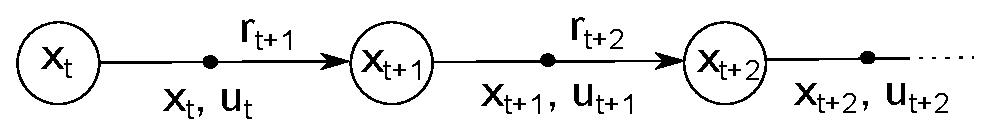
\includegraphics[width=0.7\linewidth]{sarsa}
%}
		\draw node[circle,minimum size=1cm, draw=black, line width=0.8pt] at (0,0) (circ1) {$x_t$};
		\draw node[circle,minimum size=1cm, draw=black, line width=0.8pt] at (3,0) (circ2) {$x_{t+1}$};
		\draw node[circle,minimum size=1cm, draw=black, line width=0.8pt] at (6,0) (circ3) {$x_{t+2}$};		
		\draw node[circle,scale=0.3, fill] at (1.5,0) (dot1)  {};
		\draw node[circle,scale=0.3, fill] at (4.5,0) (dot2) {};
		\draw node[circle,scale=0.3, fill] at (7.5,0) (dot3) {};
						
		\draw[line width=0.7pt, decoration={markings,mark=at position 1 with {\arrow[ultra thick]{>}}}, postaction={decorate}] (circ1) -- node[auto] {$x_t, \hspace{1mm} u_t $} (circ2);
			
		\draw[decoration={markings,mark=at position 1 with {\arrow[ultra thick]{>}}}, postaction={decorate}, line width=0.7pt] (circ2) -- node[auto] {$x_{t+1}, \hspace{1mm} u_{t+1} $} (circ3);				
		
		\draw [line width=0.7pt] (circ3) -- node[auto, pos=1.2, line width=0.8pt] {$x_{t+2}, \hspace{1mm} u_{t+2} $} (dot3);			
		\draw [dot diameter=0.8pt, dot spacing=5pt, dots] (dot3) -- ++ (1,0);
		
		\node[draw=none] at (1.5,-0.4) {$ r_{t+1} $};
		\node[draw=none] at (4.5,-0.4) {$ r_{t+2} $};
		\node[draw=none] at (7.5,-0.4) {$ r_{t+3} $};
		
		\end{tikzpicture}
		\caption{A sequence of state and action (diagram reproduced from\cite{sutton1998reinforcement})}
		\label{fig:sarsa}
	\end{figure}
	
	\begin{algorithm}[H]
		%	\KwData{this text}
		%	\KwResult{how to write algorithm with \LaTeX2e }
		\textbf{Initialization:} Initialize $ Q(x,u) $ arbitrarily\\
		\Repeat( for each episode:){episodes run out}{
			Initialize $ x $ \\
			Choose $ u $ from $ x $ using policy derived from $ Q $ \\
			\Repeat ( for each step of episode:){s is terminal}{
				Take action $ u $, observe $ r $, $ x' $ \\
				Choose $ u' $ from $ x' $ using policy derived from $ Q $ \\
				$ Q(x,u) \leftarrow Q(x,u) + \alpha[r+\gamma Q(x',u')-Q(x,u)] $	\\
				$ x \leftarrow  x' $\\
				$ u \leftarrow  u' $
			}
		} 		
		\label{alg:sarsa}
		\caption{\acs {SARSA} algorithm}
	\end{algorithm}
	
	\subsubsection{\acs{SARSA} + \acs{PID} controller}
	To incorporate \acs{SARSA} for gain scheduling purpose, we define the policy $\pi$ as the \acs {SAM} modifier (see Figure~\ref{fig:dynamictuning}) instead of the control input generator. This modification can be, for instance, in the form of the gains' probability density mean \cite{Sedighizadeh2008}. The \acs {SAM} will subsequently generates the controller parameters e.g. $ K_p $ $ K_i $ and $ K_d $ gains for \acs{PID} controller. In each iteration $\pi$ will be improved by observing the most-updated value function $Q$. Furthermore, the performance of the \acs {RL}-tuned controller needs to be evaluated in every $ N $-steps to see if the method is actually improving the tracking performance. One possible measure for evaluation is the \ac {ISE}
	\begin{equation}
	ISE = \sum_{k=0}^{N}e(k)^2 = \sum_{k=0}^{N}(y_d(k) - y_m(k))^T(y_d(k) - y_m(k))
	\end{equation}
	where $y_d$ and $y_m$ denotes desired and measured output respectively. It is also suggested to evaluate the value at each time step $Q(x(k), u(k))$. A more concrete example of a \acs{PID} controller for a linear discrete time system is presented in Algorithm~\ref{alg:pid_sarsa}.
	
	\begin{algorithm}[h]
		%	\KwData{this text}
		%	\KwResult{how to write algorithm with \LaTeX2e }
		\textbf{Initialization:} Initialize $ Q $\\
		\For{j = 1 to $ N_{episode} $}{
			Initialize $ x_0 $ \\
			\For{$ k=0 $ to $ N_{steps}-1 $}{
				\vspace{5mm}
				\textit{Compute \acs{PID} gains, error, and control input} \\
				$ K_p, K_i, K_d = \pi(x(k)) $ \\
				$ e(k) = y_d(k) - y_m(k) $ \\
				$ u(k) = K_pe(k) + K_i\sum_{i=0}^{k}e(k) + K_d[e(k)-e(k-1)]  $\\
				\vspace{5mm}		
				\textit{Update state and output} \\
				$ x(k+1) = Ax(k) + Bu(k) $\\
				$ y(k+1) = Cx(k+1) + Du(k+1) $\\				
				\vspace{5mm}
				\textit{Compute immediate reward} \\
				$ r(k+1) = \rho(x(k), u(k)) = \rho(x(k+1)) $ \\			
				\vspace{5mm}
				\textit{Compute \acs{PID} gains, error, and control input for the next time instance} \\
				$ K_p, K_i, K_d = \pi(x(k+1)) $ \\
				$ e(k+1) = y_d(k+1) - y_m(k+1) $ \\
				$ u(k+1) = K_pe(k+1) + K_i\sum_{i=0}^{k}e(k+1) + K_d[e(k+1)-e(k)]  $ \\
				\vspace{5mm}
				\textit{Update value functio}n \\
				$ Q(x(k), u(k)) \leftarrow Q(x(k), u(k)) + \alpha[r(k+1)+\gamma Q(x(k+1), u(k+1))-Q(x(k), u(k))] $	\\
				\vspace{5mm}
				modify $ \pi $ based on $ Q(x(k), u(k)) $
			}								
		}						
		\caption{\acs{PID} gain scheduling with \acs {SARSA}}
		\label{alg:pid_sarsa}
	\end{algorithm}
	

\subsection{Gain scheduling with \acs{PI$^2$}}
The second method of dynamic tuning is inspired by the sophisticated motor control of living animals. Biological motor control has shown superiority in terms of versatility and robustness to adapt to different task scenarios. Researchers have been trying to transfer the same capability to robots through variable impedance control. This task requires gain scheduling which, in one way, can be achieved by \acs{PI$^2$} algorithm. One of the main advantage of \acs{PI$^2$} is the scalability for robots with high \acs {DoF}. Although variable impedance control is the only application of \acs{PI$^2$} for robotics so far \cite{Buchli2010}, \cite{Buchli6037312}, \cite{buchli2011learning}, the method seems to be suitable for tracking application as well. Before moving on the motivation of such argument, we will summarize the \acs{PI$^2$} algorithm and its application for variable impedance control first.    

Let a continuous-time (non)linear dynamics described as 
\begin{equation}
\dot{x_t} = f(x_t) + G(x_t)(u_t + \epsilon_t)
\end{equation}
where $ G(x_t) \in \mathbb{R}^{n \times m }$ is the control matrix and $ \epsilon_t  \sim (0, \Sigma_{\epsilon}) $ is a zero-mean random variable. The key prerequisite before applying \acs{PI$^2$} is to transform the model-based stochastic optimal control problem into an approximation path integral problem. The goal of stochastic optimal control is to find an optimal input which minimizes a finite horizon cost function

\begin{equation}
J_{t_i} = V(X_{t_i}) = \underset{u_{t_i:t_N}}{\text{min}} e_{\tau_i}[R(\tau_i)]
\end{equation}
with 
\begin{equation}
R(\tau_i) = \phi_{t_N} + \int_{t_i}^{t_N}r_t dt
\end{equation}
where $ \phi_{t_N} $ is the terminal reward received at time $ t_N $ and $ \tau_i $ is a trajectory starts at time $ t_i $ and finishes at time $ t_N $. The immediate reward can be formulized as
\begin{equation}
r_t = r(x_t, u_t) = q_t + \frac{1}{2}u_t^TRu_t
\end{equation}

with $R>0$ and $q_t = q(x_t) $ is an arbitrarily chosen function, providing a degree of freedom in specifying the cost. Next, we derive the \ac {HJB} equation according to  \cite{stengel1994}

\begin{equation}
\partial _tV_t = q_t + (\partial _xV_t)^Tf(x_t)-\frac{1}{2}(\partial _xV_t)^TG_tR^{-1}G_t^T(\partial _xV_t) + \frac{1}{2}trace((\partial _{xx}V_t)G_t\Sigma_{\epsilon}G_t^T)
\end{equation}

where $ \partial _x $ and $ \partial _{xx} $ denotes jacobian and hessian respectively. Furthermore, we introduce assumptions that value function can be transformed into a logarithmic function $V_t = -\lambda$log$\Psi_t$ and $\lambda G_tR^{-1}G_t^T = G_t\Sigma_{\epsilon}G_t^T = \Sigma(x_t) = \Sigma_t$, which give us
\begin{equation}
-\partial _t\Psi_t = -\frac{1}{\lambda}q_t\Psi_t+ f(x_t)^T(\partial _x\Psi_t) + \frac{1}{2}trace((\partial _{xx}V_t)G_t\Sigma_{\epsilon}G_t^T)
\label{eq:kolmo_pde}
\end{equation}
In order to solve the so called Kolmogorov backward \ac {PDE} \eqref{eq:kolmo_pde}, we need to use Feynman Kac formula which provides a numerical approximation of the solution. The detailed derivation can be seen in \cite{oksendal2010} and \cite{5509336}. The solution of \eqref{eq:kolmo_pde} becomes
\begin{equation}
\Psi_{t_i} =  \underset{dt \leftarrow 0}{\text{lim}} \int p(\tau_i|x_i)exp \left[ -\frac{1}{\lambda}\left( \psi_{t_N} + \sum\limits_{j=0}^{N-1}q_{t_j}dt\right)\right] d\tau_i 
\label{eq:pathintegral} 
\end{equation}
Equation~\eqref{eq:pathintegral} is called path integral problem. The optimal control input can be derived:

\begin{equation}
\begin{split}
u_{t_i} &= \int P(\tau_i) u(\tau_i) d\tau_i \\
u(\tau_i) &= R^{-1}G_{t_i}^T(G_{t_i}R^{-1}G_{t_i}^T)^{-1}(G_{t_i}\epsilon_{t_i}-b_{t_i}) 
\end{split}
\end{equation}

with $P(\tau_i)$ is the probability of trajectory $\tau_i$ and $b_{t_i}$ is a complex notation which is explained in \cite{5509336}. This concludes the problem formulation for the stochastic optimal control.

It turns out that the \acs{PI$^2$} algorithm can be casted into the stochastic optimal control problem with parameterized control policy expressed as follows
\begin{equation}
a_t = g_t^T(\theta+\epsilon_t)
\end{equation}
One of the example of trajectory generator with parameterized policy is \acs {DMP} \cite{ijspeert2002learning}. The \acs{DMP} generates desired trajectory with a point of attractor $g$ and initial state $q_0$. The dynamics of \acs {DMP} is given as follows
\begin{align}
\frac{1}{\tau} \dot{v}_t &= f_t + g^T_t(\theta+\epsilon_t) \\
\frac{1}{\tau} \dot{q}_{d,t} &= v_t \\
f_t &= \alpha(\beta(g-q_{d,t})-v_t)\\
\frac{1}{\tau}\dot{s}_t &= -\alpha s_t\\
[g_t]_j &= \frac{w_js_t}{\sum_{k=1}^{p}w_k}(g-q_0)\\
w_j &= \text{exp}(-0.5h_j(s_t-c_j)^2)\\
\end{align}

The \acs{PI$^2$} algorithm will learn the optimal parameter $\theta$ which yields the optimal smooth trajectory so that the robot will go through a via-point $g$. The particular applications of such behavior are to enable robots performing task like swinging, catching, etc. The simulation and practical results presented on \cite{Buchli2010} and \cite{Buchli6037312} provide an example of an intermediate goal $g$ which the robot initially can not reach. After a number of iterations, the \acs{PI$^2$} algorithms finally manages to generate the optimal trajectory which enables to robot to reach $g$. The results also shows that \acs{PI$^2$} performs superior compared to standard \acs {RL} algorithms. This property of \acs{PI$^2$} with \acs {DMP} is interesting for tracking application if the points of attractor could be extended to a complete trajectory. To the best of author's knowledge, there is still no paper which gives the application reference tracking. Therefore, this method is one of the possible solutions for the thesis problem.

\section{Nonlinear Input Compensation via Reinforcement Learning} \label{sec:nl_comp}
The third method is a relatively new solution originated from \acs {DCSC}. As the name suggested, the idea is to learn an additive compensator to the reference signal by means of \acs{RL}. The proposed method is slightly different from the one presented in \cite{Efe2014} in the sense that the compensator is added directly to the reference signal $q_{ref}$ instead of the controller output $ u $. Furthermore, we specifically choose standard actor-critic \acs{RL} instead of \ac{MLAC} since we are not interested in learning the system model online for the sake of safety. The simplified block diagram of the control scheme is shown in Figure~\ref{fig:blockdiagram}. 

\subsection{Actor-critic formulation}
First, we need to parameterize the actor and critic using \ac {LLR} approximation \cite{Grondman6096441}. The actor and critic becomes $\pi(x_k,\vartheta_{k-1})$ and $V(x_k,\theta_k)$ respectively. As previously explained in Algorithm~\ref{alg:actorcritic}, the actor-critic will update the parameters $\theta$ and $\vartheta$ at each iteration. The fact that it uses partial derivative of value function makes actor-critic belongs to the so called policy gradient methods. Secondly, we propose the cost function as
\begin{equation}
r_k = \rho(y_m(k), y_d(k), u(k)) = (y_d(k) - y_m(k))^TQ(y_d(k) - y_m(k)) + u(k)^TRu(k)
\end{equation}
with $ Q \geq 0 $ and $ R>0 $ which is similar to that of \acs {LQT}. The possibility for a different cost function is very likely since choosing the suitable cost function itself is not a trivial problem.


\begin{figure}[h]
	\centering
	\includegraphics[width=0.8\linewidth]{nonlin_compensator.pdf}
	\caption{Block diagram of robot with \acs{RL} block acting as an additive compensator}
	\label{fig:blockdiagram}
\end{figure}

\subsection{\acs{LLR} Function Approximator}
The function approximator is needed since we are dealing with continuous state space. Popular examples of function approximator include fuzzy \cite{Efe2014}, neural networks \cite{Kiumarsi6918527} and \acs {LLR} \cite{Grondman6096441}. In this literature study, we will consider the latter due to its relatively simple and intuitive algorithm compared those of, for instance, neural network. The idea of \acs {LLR} is to approximate a non-linear function by predicting an output $\hat{y}_q$ to a certain query $x_q$ through a local fitting. This local fitting is performed by means of linear regression with respect to points $X$ which are close to $x_q$.  
The measure of distance is done by assigning weights into each point $x_i$ in the data base. 

A sorting algorithm can be employed to select $K$ number of closest neighbors from the database. Once these neighbor samples are selected, the input and output samples are said to be related with a simple linear function

\begin{equation}
Y = \beta X
\end{equation}

where 

\begin{equation}
\begin{split}
Y = \left[ \begin{array}{cccc}
y_1 & y_2 & \dots & y_K
\end{array} \right] \\
X = \left[ \begin{array}{cccc}
x_1 & x_2 & \dots & x_K \\ 
1 & 1 & \dots & 1
\end{array}  \right] 
\end{split}
\end{equation}
with the last row of $X$ is meant for bias term. The parameter $\beta$ is then computed using pseudo-inverse
\begin{equation}
\beta = YX^T(XX^T)^{-1}
\end{equation}
Now the predicted output $y_q$ can be calculated as
\begin{equation}
\hat{y}_q = \beta x_q
\end{equation}
The more samples in $X$ and $Y$, in other words the denser the neighborhood, the more accurate the prediction would be.



%\section{Iterative Learning Control} \label{sec:ilc}
%This is third section.

%\subsection{Case Study: 1-DOF Robot Gravity Compensation}


\chapter{Experimental Setup} \label{chap:testbed}

The purpose of this chapter is to present the 3D printing robot system used as the testbed. The robotic system consists of a UR5 robot manipulator, 3D print head, and a laser scanner -- each will be described in Section~\ref{sec:ur5}. In Section~\ref{sec:current_work}, we will discuss the previous works done on the robotic system. This includes the system identification model and the \ac {MPC} controller. Finally, based on the errors, we will formalize the hypothesis in Section~\ref{sec:hypo}.
\section{The 3D Printing Robot System} \label{sec:ur5}
\subsection{UR5 Robot Arm} \label{subsec:ur5}
UR5 is a lightweight, flexible industrial robot from Universal Robots. The robot is chosen due to its human-safe operation with a quite good repeatability of 0.1 mm \cite{UR5}. The robot is a serial link 6 \ac{DoF} manipulator with internal controller to take care of the gravity compensation and most of the non-linearities. In general, the robot can be controlled like a system of 6 decoupled servos, although this is only correct to some degree. We will see later why this is the case. Since the internal controller can not be "seen", let alone modified, the UR5 and the controller are viewed as one system. 

The \ac {RL} controller will be implemented in MATLAB which communicates with the UR5 using a TCP/IP protocol on 125 Hz frequency. There is a number of ways to send control command to the robot:
\begin{enumerate}
\item Tool position commmand \\
The tool position means the position of the robot's end effector in Cartesian coordinate. The origin of the Cartesian frame is exactly at the robot's base. Figure~\ref{fig:UR5_Robot01} shows a full posture of the UR5 robot. With this type of control input, one can command the end effector to move to a specified tool position $ s = (x, y, z) $ in mm. This type of command results in a smooth motion if applied in a long sampling period (> 1 second). For the 125 Hz communication rate, however, it suffers from a poor jitter.

\item Tool speed command \\
The tool speed command is in the same coordinate as the position command, but now the control input is the velocity of the end effector in mm/s. This command results in a much smoother motion compared to position command.

\item Joint position command \\
This command controls the joint position of individual robot's joint to a specified angle in radian. Similar to tool position command, it results in a jerky motion. 

\item Joint speed command \\
This command drives the individual joint into the desired joint velocity in the unit of radian/s. This results in the smoothest motion compared to others. Due to this reason, this command will be used to drive the robot throughout the thesis.

\begin{figure}
\centering
\includegraphics[width=0.5\linewidth]{UR5_Robot01}
\caption{The UR5 Robot (photo courtesy of Universal Robots)}
\label{fig:UR5_Robot01}
\end{figure}
 
\end{enumerate}

\subsection{Laser Scanner}
The laser scanner is a scanCONTROL 2700-25 series laser manufactured by Micro-Epsilon and mounted on the robot's end effector. It offers a 100 Hz profile frequency, up to 64,000 measuring points per second and 4 $ \mu $m scanning resolution. The laser scanner is used to generate the 3D point cloud of the surface we would like to print on and to measure the tracking accuracy. Figure~\ref{fig:scanCONTROL} shows the 3D view of the laser scanner.

\begin{figure}
	\centering
	\includegraphics[width=0.5\linewidth]{scanCONTROL}
	\caption{scanCONTROL 2700 series laser scanner (photo courtesy of Micro-Epsilon)}
	\label{fig:scanCONTROL}
\end{figure}

\subsection{3D Print head}
The 3D print head is a Cobalt C29 inkjet printhead developed by Oc{\'e} Technologies B.V.  Since the print head does not contribute to the controller design and implementation, it will not be used throughout the thesis. Figure~\ref{fig:ur5-endeffector} shows the robot's end effector with print head attached \cite{sunniva2013}.


\begin{figure}
\centering
\includegraphics[width=0.5\linewidth]{ur5}
\caption{The end effector of the UR5 robot with 3D print head and laser scanner attached (photo courtesy of Sunniva Ipenburg)}
\label{fig:ur5-endeffector}
\end{figure}

\section{Previous Work} \label{sec:current_work}
In this section, we will present a short overview of the previous works done by de Gier from \ac {DCSC}, specifically on the system identification and the \ac {MPC} controller \cite{Gier2013}.

\subsection{System Identification}
An important assumption for the identification is that the robot acts as six decoupled servos along with their internal controller. Additionally, it is also assumed that each joint is a \ac{LTI} system. This implies that there will be six individuals \ac {LTI} model to identify. Each model is a \ac{SIMO} system with the joint velocity reference $\dot{\theta}_r$ as the input and joint position $\theta$ and velocity $\dot{\theta}$ as the outputs. 

For this purpose, a subspace identification method is used. According to the significant singular values, the order of each model is determined to be either 4 or 5 \cite{verhaegen2007filtering}. After the models are obtained, each joint model is then validated using a square input signal while the other joint angles are held constant. The \ac{VAF} values of each joint for the validation test is shown in Table~\ref{tab:vaf}. Although the result shows a quite good \ac {VAF} score, it is still not good enough to achieve a perfect tracking. To give an example of the performance, the model validation plot of joint 1 and 5 is shown in Figure~\ref{fig:idenJoint}.

\begin{table}
\caption{\ac {VAF} scores of the simulated outputs for all joints}	
	\centering
	\begin{tabular}{|c|c|c|}
		\hline Joint & Position  & Velocity \\ 
		\hline 1 & 98.64 & 87.33 \\ 
		\hline 2 & 98.05 & 88.33 \\ 
		\hline 3 & 98.55 & 88.47 \\ 
		\hline 4 & 98.97 & 89.50 \\ 
		\hline 5 & 99.46 & 90.32 \\ 
		\hline 6 & 98.87 & 85.13 \\ 
		\hline 
	\end{tabular} 
	\label{tab:vaf}
\end{table}


\begin{figure}
	\centering
	\begin{subfigure}[b]{0.4\textwidth}
		\includegraphics[width=1\linewidth]{"../../Progress Report/Joint5"}
		\caption{}
		\label{fig:Joint5}
	\end{subfigure}%
	~ %add desired spacing between images, e. g. ~, \quad, \qquad, \hfill etc.
	%(or a blank line to force the subfigure onto a new line)
	\begin{subfigure}[b]{0.4\textwidth}
		\includegraphics[width=1\linewidth]{"../../Progress Report/Joint1"}
		\caption{}
		\label{fig:Joint1}
	\end{subfigure}
	\caption{Model validation of joint 1 and 5 for joint position and velocity}\label{fig:idenJoint}
\end{figure}

\newpage
\subsection{\ac{MPC} Controller}
The previous work involves a design and implementation of \ac {MPC} controller. As the comparisons, we will control the robots using 3 of the 4 methods described in Subsection~\ref{subsec:ur5}: tool position, tool velocity and joint velocity command. We will call these three control methods the default controllers. The experiment is to make the robot following a straight line along X-axis with constant values on Y and Z axes.  In order to see the effect of robot's speed to the errors, the experiment is repeated with three different speeds for the default controllers. As for the \ac {MPC}, only one speed is possible due to the difficulty to modify the provided \ac {MPC} program. The plots for Y and Z trajectories are shown in Figure~\ref{fig:trajectory_data_Y} and \ref{fig:trajectory_data_Z} respectively. 

As we can see, there is a shaky behavior in both axes trajectories. To have an idea of how large the amplitude of the jitter, we calculate the difference between maximum and minimum values of each trajectory as shown in Table~\ref{tab:y_jitter} and \ref{tab:z_jitter}. The Y-axis trajectory for the default controllers are slowly drifting from the desired value. This is expected since the default controllers are basically open loop controllers. This causes the jitter's amplitude to be much higher than the \ac {MPC} (see Table~\ref{tab:y_jitter}). Furthermore, for different speeds, the jitters of each default controller behave similarly. If we run the controller for several iterations at constant speed, the plot (not shown here) confirms that the jitter indeed shows a repeating behavior. 

Table~\ref{tab:y_jitter} has shown that the \ac {MPC} controller manages to reduce the jitter significantly -- it almost reaches the robot repeatability. However, for The Z-axis trajectory, the jitter is much larger. 

\begin{table}
	\centering
	\caption{The difference between maximum and minimum values of Y-axis trajectory with different control methods}
	\begin{tabular}{|c|c|c|}
		\hline
		Control method & speed & jitter's amplitude (mm) \\
		\hline		
		& $ \times $1 & 0.635678\\
		Tool Position & $ \times $2 & 0.670974\\
		& $ \times $4 & 0.624456\\
		\hline		
		& $ \times $1 & 0.529104\\
		Tool Velocity & $ \times $2 & 0.376090\\
		& $ \times $4 & 0.320906\\
		\hline		
		& $ \times $1 & 0.550691\\
		Joint Velocity & $ \times $2 & 0.522474\\
		& $ \times $4 & 0.490630\\				
		\hline
		\ac {MPC} & $ \times $1 & 0.120889 \\
		\hline

	\end{tabular}
	\label{tab:y_jitter}
\end{table}

\begin{table}
	\centering
	\caption{The difference between maximum and minimum values of Z-axis trajectory with different control methods}
	\begin{tabular}{|c|c|c|}
		\hline
		Control method & speed & jitter's amplitude (mm) \\
		\hline		
		& $ \times $1 & 0.879843\\
		Tool Position & $ \times $2 & 0.805172\\
		& $ \times $4 & 0.800554\\
		\hline		
		& $ \times $1 & 0.904581\\
		Tool Velocity & $ \times $2 & 0.909465\\
		& $ \times $4 & 1.007834\\
		\hline		
		& $ \times $1 & 0.793960\\
		Joint Velocity & $ \times $2 & 0.795276\\
		& $ \times $4 & 0.975885\\				
		\hline
		\ac {MPC} & $ \times $1 & 0.795315 \\
		\hline
		
	\end{tabular}
	\label{tab:z_jitter}
\end{table}

%\begin{figure}
%\centering
%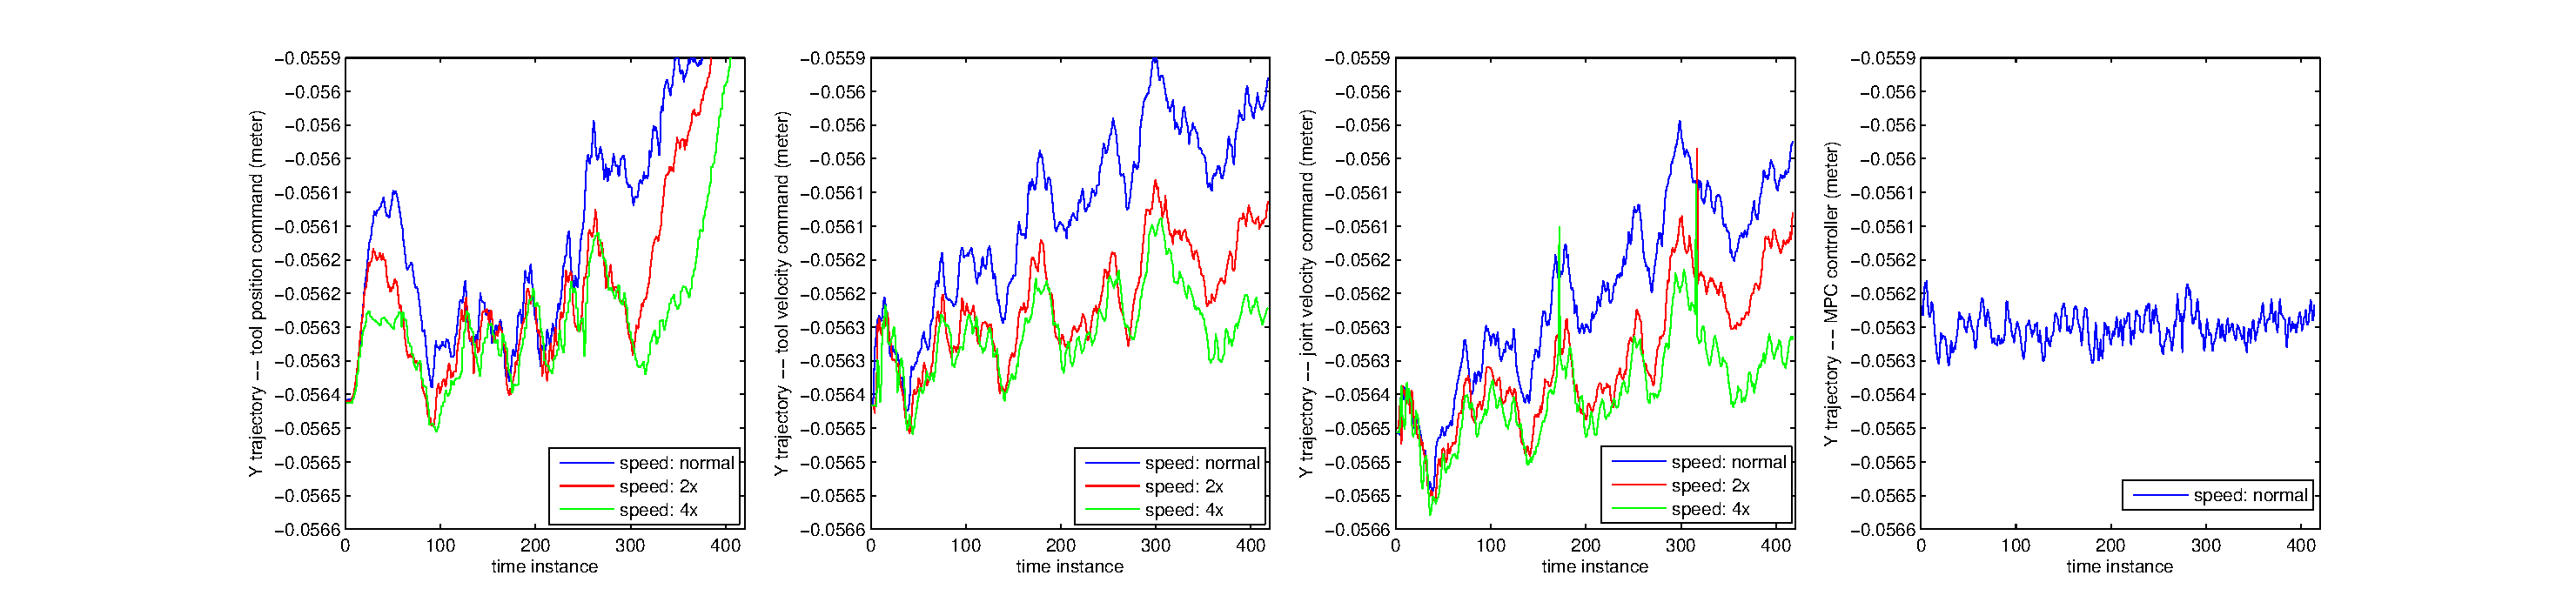
\includegraphics[width=0.7\linewidth]{trajectory_data_Y}
%\caption{the Y trajectories of the robot with different controllers. From left to right: tool position command, tool velocity command, joint velocity command and \ac{MPC}}
%\label{fig:trajectory_data_Y}
%\end{figure}
%\begin{figure}
%\centering
%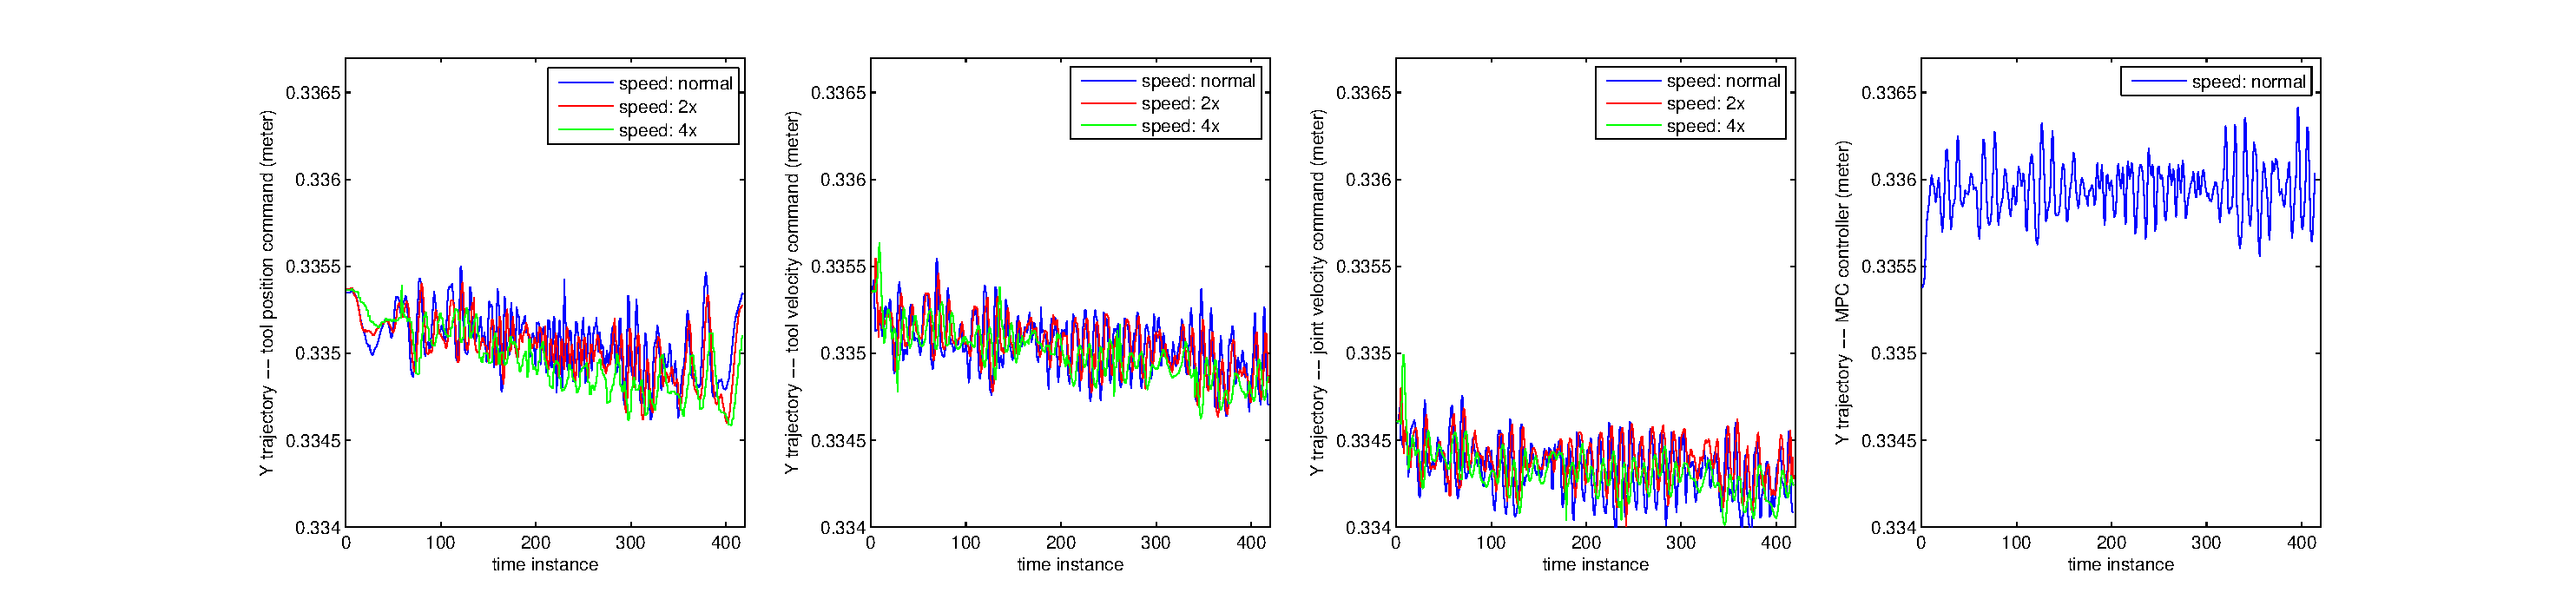
\includegraphics[width=0.7\linewidth]{trajectory_data_Z}
%\caption{the Z trajectories of the robot with different controllers. From left to right: tool position command, tool velocity command, joint velocity command and \ac{MPC}}
%\label{fig:trajectory_data_Z}
%\end{figure}

 


\chapter{Research Direction and Discussion}

This chapter presents the result of the literature study. It starts in Section~\ref*{sec:review} by presenting the review and analysis of the three \ac {RL} approaches explained in Chapter~\ref{chap::survey}. The review consists of parameters that are taken into considerations -- advantages, limitations and practical challenges for implementation. Section~\ref{sec:res_planning} presents the research plan which will be carried out during the thesis. In the end of the chapter, a discussion is covered in Section~\ref{sec:discussion}
\section{Review and Analysis of \ac{RL} Approaches} \label{sec:review}
\subsection{{\ac{RL} for Optimal Tracking Control}}
From the mathematical perspective, the optimal tracking approach is more rigorous compared to the other two. The proof of convergence, for instance, has been provided in literature \cite{1099755}. Another advantage is since the approach is based on lyapunov function, system's stability is guaranteed. Furthermore, researchers have successfully extended this approach to different control condition: discrete-continuous time, linear-nonlinear system, known-(partially)unknown model. From all of these benefits, the optimal tracking approach seems to be a suitable choice. However, there are some limitations which must be overcome in order to implement this method for a robotic tracking application.

As previously stated in the motivation, the goal of the thesis is to push the envelope of current tracking performance using \ac {RL}. As for the case-specific, it is hypothesized in Chapter~\ref{chap:testbed} that the low tracking performance is due to unknown non-linearities and disturbance in the robot. Therefore, a model-based standard optimal tracking is no longer a relevant solution. Although \cite{Kiumarsi20141167} has shown that using \ac{RL}, one can obviate the need of system model for linear system, the solution for an unknown non-linear system is not yet available. This is one crucial limitation to this method for now since we actually want to improve tracking of potentially non-linear system. Even if the solution exists, a practical problem will most probably arise due to the necessity of persistence of excitation in order to achieve a converging control policy \cite{Kiumarsi20141167} \cite{AlTamimi2007473}. For the UR5 robot testbed, this could potentially damage the robot since the motors must be excited with a persistently exciting signal such as pseudo-random noise. 

The second limitation of the approach is that it is still not known how to integrate the available but inaccurate model to the optimal tracking. Literatures have shown that although the models are not perfect, it can still help in speeding up the \ac {RL} convergence time \cite{Brujeni5669655} \cite{Grondman6096441}. Therefore, model integration would be a useful, though not necessary factor. Due to these factors, optimal tracking \ac {RL} is not the most suitable method for the thesis requirements.

\subsection{Dynamic Tuning via \ac{RL}}
\subsubsection{Direct Tuning of Nominal Controller}
The advantage of the direct tuning by \ac{RL} is its simple, intuitive scheme and rather direct implementation. However, direct tuning \ac{RL} only works with a standard state/output feedback controller such as \ac{PID}. State/output feedback controller is known for its nature which is always "late" since it has to wait for the error to appear and then compensate for it. Throughout the literature survey, author could not find a paper which integrates an \ac{RL}-based dynamic tuning with more sophisticated controller such as optimal tracking control or \ac {MPC}. Due to this bottleneck in performance, the direct-tuning is not the best choice to answer the research's goal.
\subsubsection{Gain scheduling for \ac{DMP}}
As previously explained in Chapter~\ref{chap::survey}, \ac{PI$^2$} learns the optimum trajectory to enable robotic manipulator passing through a certain intermediate point described by \ac{DMP}. In order to use \ac{PI$^2$} \ac{DMP} for reference tracking, one would need to extend the point of attractor $g$ into a full trajectory $g(k)$. The answer of this problem, assuming that the question itself is relevant, is not present at this time.

In order to provide an answer to above problem, a thorough understanding of the \ac{PI$^2$} algorithm and \ac {DMP} approach is needed. This is a particularly challenging problem since to derive the \ac{PI$^2$} itself involves a rather complex procedures such as stochastic optimal control which can easily be misunderstood if not treated carefully \cite{Buchli2010}. Due to the needs of extensive theoretical study, duration constraint of the thesis and the risk that this method is ultimately irrelevant, it is decided that \ac {PI$^2$} \ac{DMP} is not the most suitable solution.

\subsection{Nonlinear Input Compensation via \ac{RL}}
To the best of author's knowledge, there is no any literature yet which addresses the implementation of this method to a full reference tracking task. The only existing work is presented in \cite{Efe2014} which compensates an unknown gravity for a \ac {PD}-controlled 1-\ac {DoF} robot arm acting on a simple step command. Thus, this method, if successfully implemented, can be considered a novel solution. This algorithm is also modular in the sense that the compensator acts as an additive signal which does not influence the controller's output. This means the better the nominal controller performs, the smaller tracking errors needs to be compensated. Furthermore, the compensator also does not require any information about the system model to operate. 

The drawback of this method is the lack of mathematical formalization to prove the common control criterion: stability, convergence and robustness. From the practical point of view, some kind of mechanism must be introduced to ensure that the compensator signal is not too large since the nominal controller has already performed near optimally. Nevertheless, due to the model-free characteristic, this method is chosen to be the solution which will be developed and implemented for the rest of the thesis.

\section{Research Plan} \label{sec:res_planning}
The post-literature survey research plan is organized as follows. Before commissioning the implementation on the UR5, a simple simulation of a 1-\ac {DoF} manipulator will be programmed. The purpose of the simulation is to verify that the proposed method is actually working. If the \ac{RL}-based optimizer indeed works, the next step would be to further develop the controller for implementation on the UR5 robot. If the controller performs as expected, improvement will be carried out until the end of the thesis. Parallel to these steps, the thesis report will be written as well. The research plan is summarized in a flowchart as shown in Figure~\ref{fig:flowchart}.

\begin{figure}
\centering
\includegraphics[width=0.5\linewidth]{Drawing1}
\caption{Research plan flowchart}
\label{fig:flowchart}
\end{figure}

%\section{Discussion}\label{sec:discussion}
%During the implementation, 

\chapter{Conclusion}
Despite having used for various applications for decades, the application of \ac {RL} in control still has much space to explore. In this thesis, a subset of that space, namely reference tracking problem is addressed. The search for existing works results in 3 methods which must be analyzed carefully in order to obtain a strong motivation to finally choose one of them. The \ac {RL}-based optimal tracking is mathematically more convincing than the other two. Not only that it will surely converge, a stability can also be guaranteeed. In the other hand, the dynamic tuning methods have problems with performance and feasibility. The direct tuning is intuitive and relatively easy to implement, but it will perform less since it depends on a feedback controller which will always be late in compensating error. The \ac{PI$^2$} method has successful track-record for variable impedance control task, but rather unconvincing for tracking problem. Finally, the additive tracking problem is chosen since it strongest represents the nature of \ac {RL} which does not depend on the system model. This method enables an additional degree of freedom to optimize the controller, independent from the nominal controller itself. Furthermore, it is considered interesting to compare the \ac{RL}-based tracking controller with a more widely known \ac{ILC}.
%
%
%========================== Appendices =======================================
\appendix
%
%\chapter{Appendix}

Appendices are found in the back. 

\section{Simulation Program}

\subsection{A MATLAB listing}

\lstset{language=matlab}
\lstinputlisting{test.m}


%========================== Back matter ======================================
\backmatter
%
% Bibliography
\bibliographystyle{ieeetr}
\bibliography{MyBib}

%
%
% Glossary
\chapter{Glossary} %
%
\printacronyms
\begin{acronym}[\hspace{0.8in}] % 0.8in is also used by the nomenclature
	\acro{3D}{3-dimension}	
	\acro{3mE}[3\textlarger{m}E]{Mechanical, Maritime and Materials Engineering}%
	\acro{AMS}{American Mathematical Society}%
	\acro{ARE}{algebraic Riccati equation}	
	\acro{DCSC}{Delft Center for Systems and Control}%	
	\acro{DMP}{dynamic movement primitive}
	\acro{DoF}{degrees of freedom}%
	\acro{DP}{Dynamic Programming}
	\acro{HJB}{Hamilton-Jacobi-Bellman}
	\acro{ILC}{iterative learning control}
	\acro{ISE}{integral of squared errors }
	\acro{LLR}{local linear regression}
	\acro{LQT}{linear quadratic tracking}
	\acro{LTI}{linear time-invariant}	
	\acro{MDP}{markov decision process}%
	\acro{MIMO}{multi-input multi-output}
	\acro{MLAC}{model learning actor-critic}
	\acro{MPC}{model predictive control}
	\acro{PD}{proportional derivative}		
	\acro{PDE}{partial differential equation}
	\acro{PI}{policy iteration}	
	\acro{PI$^2$}{policy improvement with path integral}
	\acro{PID}{proportional-integral-derivative}
	\acro{RL}{reinforcement learning}%
	\acro{SARSA}{state-action-reward-state-action}
	\acro{SIMO}{single-input multi-output}
	\acro{SISO}{single-input single-output}	
	\acro{TD}{temporal-difference}	
	\acro{TU}[TU D\textlarger{elft}]{Delft University of Technology}%
	\acro{VAF}{variance accounted for}
	\acro{VI}{value iteration}
\end{acronym}%
%
%
% Nomenclature
\printnomencl%
%
% Index
\cleardoublepage
\printindex

\end{document}
